\section{Experiments}
\label{sec:4:experiments}

In this section, we first introduce the two major benchmarks ---WebArena and Mind2Web, and top-performing baselines on them (\S\ref{sec:4.1:benchmark-and-baseline}). Next, we present our \awm approach on both benchmarks, showcasing its ability to achieve task success and generalization across varied setups (\S\ref{sec:4.2:webarena-results}, \S\ref{sec:4.3:mind2web-results}).


%%%%%%%%%%%%%%%%%%%%%%%%%%%%%%%%%%%%%%%%%%%%%%%%%%%%%
\subsection{Benchmarks and Baselines}
\label{sec:4.1:benchmark-and-baseline}

\paragraph{WebArena}
% dataset
\citep{zhou2024webarena} provides 812 web navigation tasks on five websites that cover four common application domains: e-commerce, social forum discussions, collaborative software development, and content management. Most importantly, WebArena supports rigorous evaluation on the functional correctness of agent trajectories. 

% sota method
We adopt the current state-of-the-art method without human-distilled knowledge, BrowserGym \citep{drouin2024workarena}, which altered the agent action space to a set of bid-based actions. We adopt the BrowserGym framework alone with its bid-based action space, and represent webpages using accessibility trees, aligning to the environment representation in \citet{zhou2024webarena}. Because BrowserGym inputs both webpage HTML and accessibility tree representations, to keep a fair comparison with our method, we also run the BrowserGym version with only accessibility tree webpage representations, denoted as BrowserGym$_{\it ax-tree}$.
%
Note that, the SteP \citep{sodhi2023heap} method outperforms BrowserGym, yet achieves so by adding 14 human expert written workflows tailored for solving WebArena. We thus view SteP as an oracle setting and will show \awm's superior results over it.


% atm setup
Aligning with baseline approaches, we use \texttt{gpt-4} and use a temperature of $0.0$ to ensure fairly stable model outputs.
Because WebArena only contains test examples and no additional high-quality, domain-aligned examples exist, we only conduct \awm in the online setting as introduced in \S\ref{sec:3.3.2:online}.
 


\paragraph{Mind2Web}
\citep{deng2023mindweb} features web navigation tasks across a wide range of websites and domains, stressing the generalization abilities of agents over versatile operations and environments. 
Each task in Mind2Web has a fixed number of steps; at each step, the agent needs to predict an action, which is evaluated in three dimensions: (1) \textit{Element accuracy}: to check if the correct element is selected in the predicted action, (2) \textit{Action F$_1$} to check if the action taken is correct, and aggregating (1) and (2) yields, (3) \textit{Step success rate} to check if both element and action selection is correct at the current step. Lastly, after completing every step in the given task, the last metric (4) \textit{success rate} measures if all intermediate steps are successfully conducted for this task, \ie, only when all steps score 1 in metric (3) get a full score in metric (4).

Because Mind2Web provides a training set covering a portion of tested websites and domains, we explore both \textit{offline} setting that induces workflows from the training set and applies to test sets, as well as the \textit{online} setting, where we do streaming induction and inference on test queries only.

Since we focus on LM-based agents that only take textual inputs, we compare \awm to two state-of-the-art methods, MindAct \citep{deng2023mindweb} and Synapse \citep{zheng2024synapse}. MindAct introduces webpage element filtering and multi-choice task format to ease observation processing, and Synapse changes the format to a trajectory style and augments retrieved relevant examples. We integrate the element filtering adopted in both methods, and added workflows instead of retrieved examples in Synapse, to verify the superiority of reusable workflows over concrete examples. To fairly compare with all baseline methods, we run \awm with both \texttt{gpt-3.5-turbo} and \texttt{gpt-4} models.

For both datasets, we induce and incorporate workflows on a website basis. In other words, we group examples by their associated websites, and respectively run \awm on each group. We report the micro-average scores over all groups, \ie, average scores of all examples. This mechanism maintains an effectively small workflow repository, while bringing the maximum benefit to the pertinent tasks.


\subsubsection{Main results}
% \label{sec:4.2:webarena-results}

\begin{table}[t!]
\vspace{-3mm}
\centering
\small
\caption{Task success rate on WebArena using \texttt{gpt-4}, and score breakdown on five website splits.}
\vspace{2mm}
\label{tab:webarena-results}
%
\begin{tabular}{l|c|ccccc|c}
\toprule
\multicolumn{1}{c|}{\bf Method} & {\bf Total SR} & {Shopping} & {CMS} & {Reddit} & {GitLab} & {Maps} & {\bf \# Steps} \\
\midrule
\dlrow \multicolumn{8}{c}{\it With human engineered workflows} \\
{*SteP \citep{sodhi2023heap}} & {33.0} & {\bf 37.0} & {24.0} & {\bf 59.0} & {\bf 32.0} & {30.0} & {-} \\
\midrule
\dlrow \multicolumn{8}{c}{\it Autonomous agent only} \\
{WebArena \citep{zhou2024webarena}} & {14.9} & {14.0} & {11.0} & {~6.0} & {15.0} & {16.0} & {-} \\
{AutoEval \citep{pan2024autonomous}} & {20.2} & {25.5} & {18.1} & {25.4} & {28.6} & {31.9} & {46.7} \\
{BrowserGym \citep{drouin2024workarena}} & {23.5} & {-} & {-} & {-} & {-} & {-} & {-} \\
{BrowserGym$_{\it ax-tree}$} & {15.0} & {17.2} & {14.8} & {20.2} & {19.0} & {25.5} & {~~7.9} \\
\midrule
% \textsc{AWM$_{\it rule}$ (ours)} & {\bf 35.6} & {33.2} & {\bf 30.2} & {50.9} & {30.8} & {40.5} & {~~6.3} \\
\textsc{AWM (ours)} & {35.5} & {30.8} & {29.1} & {50.9} & {31.8} & {\bf 43.3} & {\bf ~~5.9} \\
\bottomrule
\end{tabular}
\vspace{-4mm}
\end{table}


As shown in \autoref{tab:webarena-results}, our \awm achieves the best published results on WebArena, surpassing the BrowserGym baseline by $12.0$ absolute points and $51.1$\% relative increase in overall success rate. Notably, \awm also outperforms SteP, which uses strong domain-specific supervision from human-written workflows, by a $7.6$\% relative increase in overall success rate.
According to the breakdown on five websites, our \awm method substantially enhances the agent performance across all websites over the BrowserGym baseline, by $11.8$--$30.7$ absolute points, indicating its general applicability across varied domains and tasks.

Beyond task success, we also evaluate the average number of steps the agent takes to solve a task, as shown in the rightmost column in \autoref{tab:webarena-results}. \awm conducts about $2.0$ fewer steps per example than the BrowserGym baseline. Further compared to the Autoeval \citep{pan2024autonomous} method, which necessitates additional evaluation and refinement steps to solve tasks correctly, our \awm approach uses $40.8$ fewer steps on average. Both comparisons show that \awm obtains high success rates while maintaining efficient trajectories.



%%%%%%%%%

\begin{wrapfigure}[15]{r}{0.5\textwidth}
\vspace{-2mm}
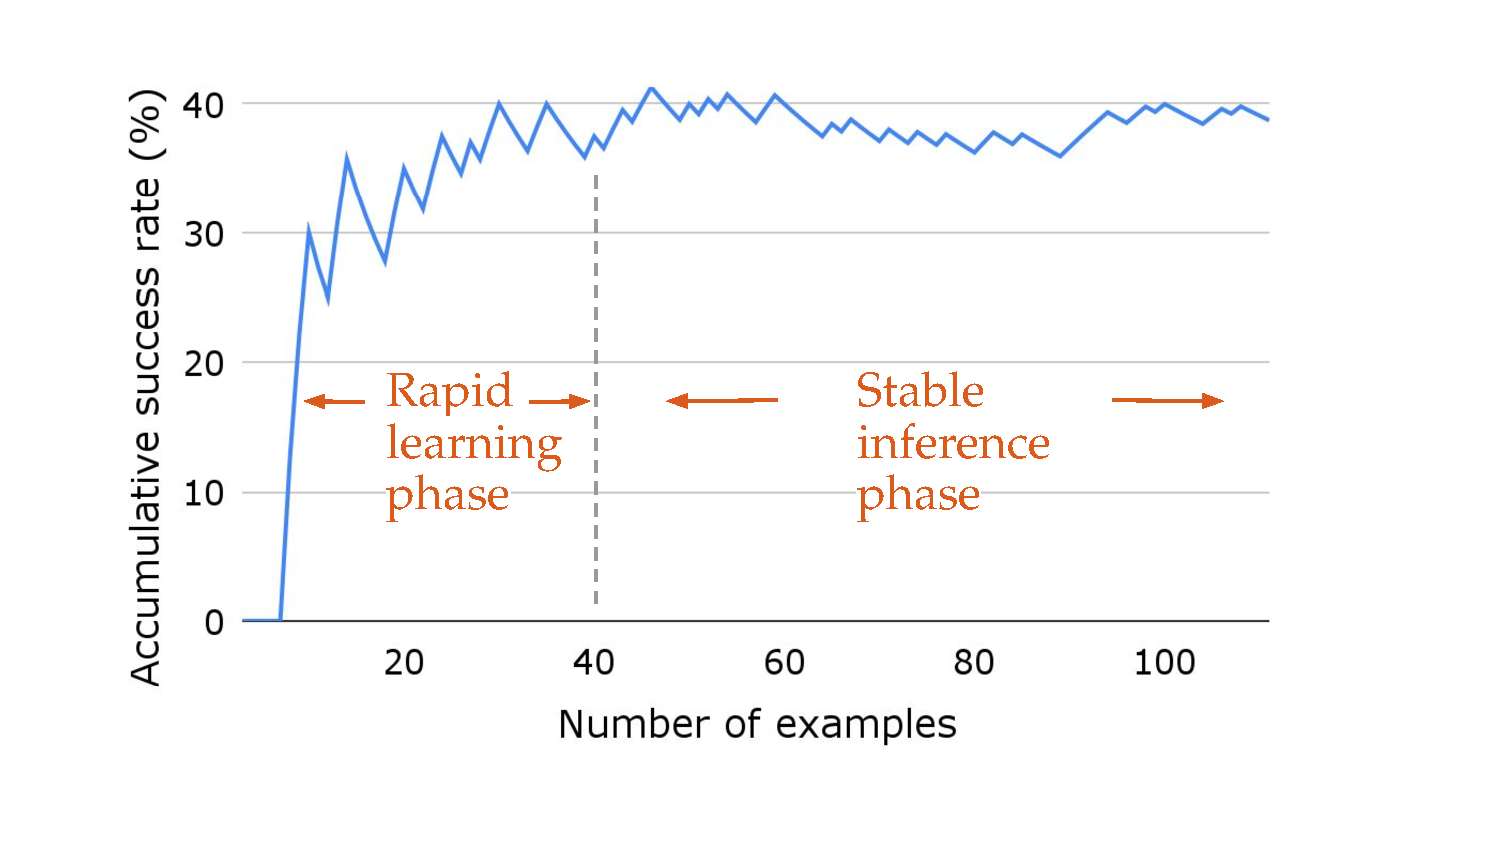
\includegraphics[width=0.49\textwidth]{./figures/webarena-learning.pdf}
% \vspace{-1mm}
\caption{\awm enables rapid learning from a small amount of data, i.e., about 40 queries, using WebArena map test split as an example.}
\label{fig:webarena-learning}
% \vspace{-1mm}
\end{wrapfigure}


%%%%%%%%%%
\subsubsection{Efficient learning from small amounts of data}
To demonstrate the behavior of the $\awm_{\it online}$ method, we illustrate the cumulative success rate over the process of online evaluation, by evaluating the average success rate of the first $k$ finished examples. 

As in \autoref{fig:webarena-learning}, the agent exhibits a fast learning curve in the beginning (between 0--40 examples), by acquiring the most essential workflows, which results in higher success rates. Afterward, agents learn more advanced workflows (\autoref{fig:teaser}), while success rates gradually stabilize to the highest point in the early learning phase.
This showcases \awm's efficient learning process, which substantially improves performance with merely tens of examples.



%%%%%%%%%%
\subsubsection{Cross-template workflow generalization}
Some tasks in the WebArena benchmark have highly overlapping canonical trajectories, due to the benchmark construction process that instantiates multiple examples from a single underlying task template. 
\awm intuitively improves in-template success rate, that is, given one workflow induced from a successful example, it would be theoretically easier to solve all other examples generated from the same task template.

To confirm that the benefits of \awm are not just from learning workflows that help only within a template, and investigate whether \awm can obtain cross-template ($\approx$cross-task) generalization, we extract a subset of WebArena examples sourcing from non-overlapping templates, by grouping examples by their templates and randomly choosing one example from each template group.
We run \awm on this cross-template subset and examine if it achieves similar performance gains.


\begin{table}[t!]
\vspace{-3mm}
\centering
\small
\caption{Task success rate on the cross-template subset of WebArena, as well as the result breakdown on each website split. We mark the number of examples for each website split under the name.}
\vspace{2mm}
\label{tab:cross-template-webarena-results}
%
\begin{tabular}{l|c|ccccc}
\toprule
\multicolumn{1}{c|}{\multirow{2}{*}{\bf Method}} & \multirow{2}{*}{\bf Total SR} & {Shopping} & {CMS} & {Reddit} & {GitLab} & {Maps} \\
{} & {} & {(51)} & {(45)} & {(24)} & {(45)} & {(32)} \\
\midrule
\dlrow \multicolumn{7}{c}{\it With human engineered workflows} \\
{*SteP \citep{sodhi2023heap}} & {32.1} & {\bf 26.5} & {\bf 29.3} & {\bf 52.2} & {27.3} & {36.4} \\
\midrule
\dlrow \multicolumn{7}{c}{\it Autonomous agent only} \\
{AutoEval \citep{pan2024autonomous}} & {23.2} & {12.2} & {17.1} & {21.7} & {\bf 31.8} & {36.4} \\
{BrowserGym$_{\it ax-tree}$} & {20.5} & {10.4} & {17.8} & {23.1} & {27.3} & {28.6} \\
\textsc{AWM (ours)} & {\bf 33.2} & {24.5} & {\bf 29.3} & {\bf 52.2} & {\bf 31.8} & {\bf 39.4} \\
\bottomrule
\end{tabular}
\vspace{-4mm}
\end{table}

As shown in \autoref{tab:cross-template-webarena-results}, \awm still achieves the highest performance, overall and on each website split. These results demonstrate that \awm induced workflows can effectively generalize across different tasks, i.e., examples instantiated from different task templates.


\begin{wrapfigure}[9]{r}{0.67\textwidth}
\vspace{-5mm}
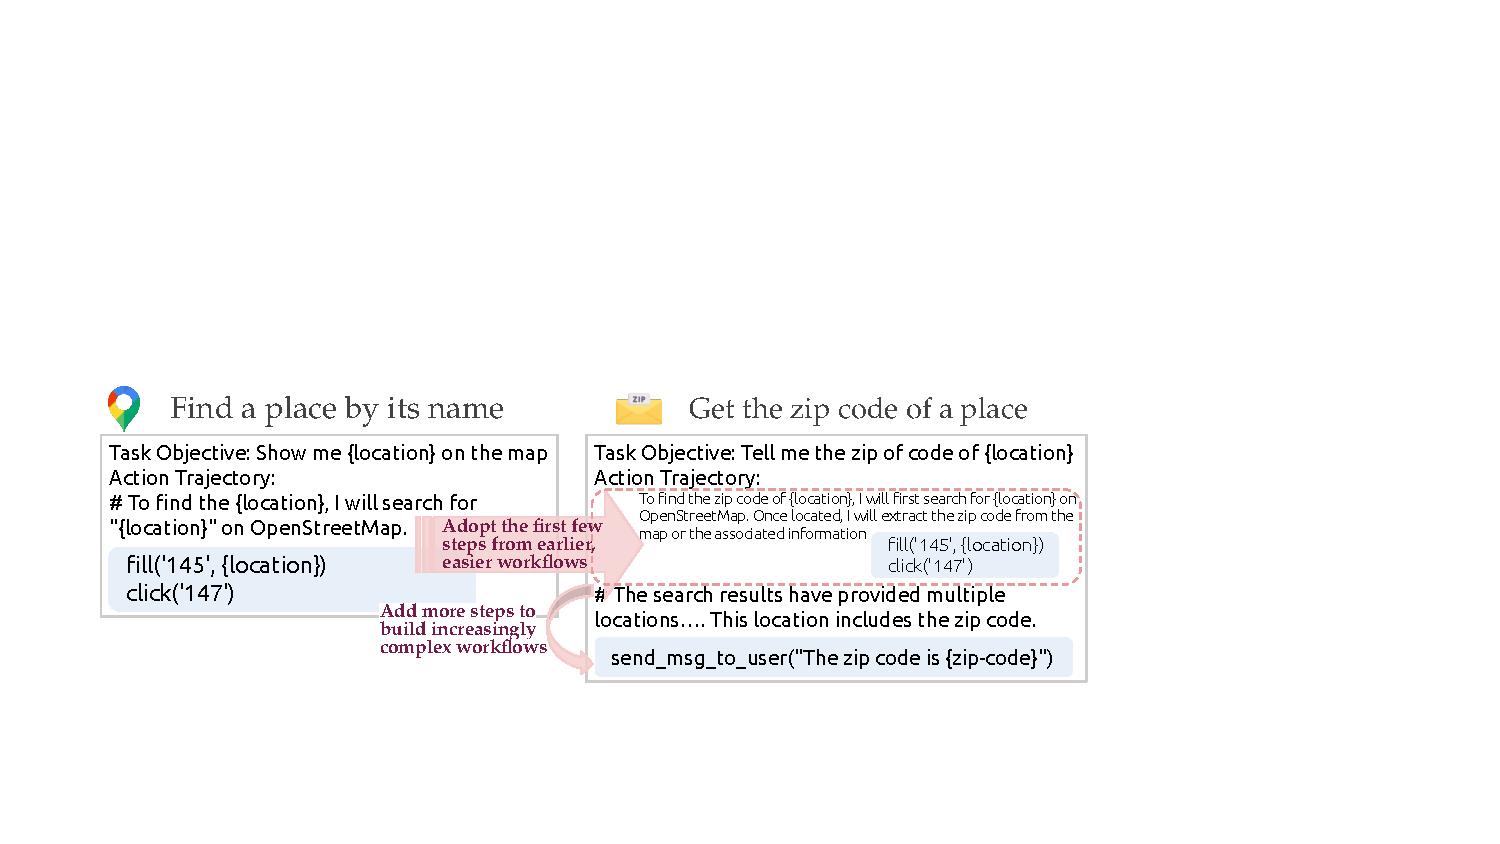
\includegraphics[width=0.67\textwidth]{./figures/complex-workflows.pdf}
\vspace{-6mm}
\caption{\awm builds increasingly complex workflows over time, by learning from past examples and earlier workflows.}
\label{fig:complex-workflows}
% \vspace{-1mm}
\end{wrapfigure}



% \noindent \textbf{Building increasingly complex workflows} \quad
\paragraph{Building increasingly complex workflows}
To more intuitively demonstrate \awm's cross-template generalization and ability to build increasingly complex workflows (as exemplified in \autoref{fig:teaser}), we conduct a case study to illustrate the workflow mechanism behind it. 

As exemplified in \autoref{fig:complex-workflows}, the agent creates and learns the ``Find a place by its name'' workflow in the early stage of the online process by summarizing past examples. Later, when encountering an example that further asks to obtain the zip code of the location, \awm agent learns to adopt the first few steps to find locations by following the existing workflow, and then conducts further steps to obtain the zip code of the place found. Integrating these new steps upon the vanilla find location task, the agent successfully builds a more complex workflow, i.e., ``get the zip code of a place''.

\subsubsection{Main results}
% \label{sec:4.3:mind2web-results}

\begin{wraptable}[14]{r}{0.55\textwidth}
\small
\vspace{-8mm}
\caption{\awm offline results on Mind2Web cross-task dataset. Elem Acc and SR are short for element accuracy and success rate. We footnote the GPT variant used by each method, \texttt{3.5} and \texttt{4} stands for \texttt{gpt-3.5-turbo} and \texttt{gpt-4}, respectively. We highlight the best result within the same model variant.}
\vspace{1mm}
\label{tab:mind2web-results}
\resizebox{0.55\textwidth}{!}{
\begin{tabular}{l|cccc}
\toprule
\multicolumn{1}{c|}{\bf Method} & {\bf Elem Acc} & {\bf Action F$_{1}$} & {\bf Step SR} & {\bf SR} \\
\midrule
MindAct$_{3.5}$ & {20.3} & {\bf 56.6} & {17.4} & {0.8} \\
CogAgent$_{3.5}$ & {-} & {-} & {18.6} & {-} \\
Synapse$_{3.5}$ & {34.0} & {-} & {30.6} & {2.4} \\
\textsc{AWM$_{3.5}$} & {\bf 39.0} & {52.8} & {\bf 34.6} & {\bf 2.8} \\
\midrule
MindAct$_{4}$ & {41.6} & {\bf 60.6} & {36.2} & {2.0} \\
% \textsc{AWM$_{4, rule}$} & {49.5} & {57.0} & {43.4} & {2.0} \\
\textsc{AWM$_{4}$} & {\bf 50.6} & {57.3} & {\bf 45.1} & {\bf 4.8} \\
\bottomrule
\end{tabular}
}
\vspace{-4mm}
\end{wraptable}

We first run with \awm offline using both GPT variants, and find that \awm consistently obtains the highest success rate in both step and task levels, leading to $4.0$--$8.9$\% relative and $0.4$--$2.8$ absolute points increases in step-wise and task-wise success rates than the baselines --- Synapse with \texttt{gpt-3.5-turbo} and MindAct with \texttt{gpt-4}. 
%
Decomposing the step success rate by element and action selection and accuracy, we notice the increases mainly come from more accurate element selection, as indicated by the $5.0$--$9.0$ element accuracy increase in \autoref{tab:mind2web-results}. 

% \noindent \textbf{Abstract sub-routines vs. concrete experiences} \quad
\paragraph{Abstract sub-routines vs. concrete experiences}
More specifically, compared to the Synapse \citep{zheng2024synapse} method that retrieves the most relevant training examples, \awm achieves a $+5.0$ element accuracy and leads to a $+4.0$ increase in step success rate.
While augmenting concrete, full examples may bias agents to select elements similar to those presented in the given examples, \awm introduces less bias on element selection via its abstract representation of example-specific contexts in workflows, and therefore enables higher step success rates.

Furthermore, \awm integrates frequently-used sub-routines, which can be more flexibly and readily leveraged across test examples, compared to the full example trajectories used by Synapse, which are less likely to appear multiple times.
In general, our results indicate that the abstract, reusable nature of workflows contributes to the superiority of the \awm method.

% \noindent \textbf{Learn to diverge from workflow guidelines} \quad
\paragraph{Learn to diverge from workflow guidelines}
Despite more accurate element selection, \awm gets slightly lower action F$_1$ scores than MindAct, possibly because the augmented workflows may guide the agent to take certain actions aligning to the workflows, which are not always relevant to the particular environment state at hand. While following the workflows generally results in more successful task trajectories, agents still encounter some challenges in identifying places to diverge from the workflow guidelines.


\subsubsection{Online \awm Enables Generalization}

Beyond the offline induction setting, we further explore the \awm in the online setting, similar to the WebArena experiment setup in \S\ref{sec:4.1:webarena}, where no additional training examples are needed besides test queries. This naturally facilitates cross-website and cross-domain generalization, which we examine on the two other splits provided by the Mind2Web dataset: cross-website and cross-domain tests. 

In addition to the MindAct baseline, we additionally set bars with our \textsc{AWM$_{\it offline}$} setup, by randomly selecting workflows induced from the training set as memory augmentations. Specifically, for cross-website examples, we select workflows from the same domain; for the cross-domain setting, we randomly select workflows from all domains.
We conduct \textsc{AWM$_{\it online}$} by iteratively inducing, integrating, and utilizing workflows over test inferences. We also explore \textsc{AWM}$_{\it offline+online}$ in \S\ref{app:mind2web-offline-online}.

As shown in \autoref{tab:mind2web-generalize}, both \textsc{AWM$_{\it online}$} and \textsc{AWM$_{\it offline}$} surpass the MindAct baseline by a large margin, resulting in $7.4$--$8.9$, $3.6$--$3.8$, and $14.0$--$16.9$ absolute point improvements in step success rates, in cross-task, cross-website, and cross-domain scenarios.


\begin{table}[t!]
\vspace{-4mm}
\small
\centering
\caption{Success rate on Mind2Web cross-task, cross-website, and cross-domain generalization test, using \texttt{gpt-4} model. EA is short for element accuracy and AF$_1$ is short for action F$_1$.}
\vspace{1mm}
\label{tab:mind2web-generalize}
\resizebox{\textwidth}{!}{
\begin{tabular}{l|cccc|cccc|cccc}
\toprule
\multirow{2}{*}{\bf Method} & \multicolumn{4}{c|}{\it Cross-Task} & \multicolumn{4}{c|}{\it Cross-Website} & \multicolumn{4}{c}{\it Cross-Domain} \\
{} & {EA} & {AF$_{1}$} & {Step SR} & {SR} & {EA} & {AF$_{1}$} & {Step SR} & {SR} & {EA} & {AF$_{1}$} & {Step SR} & {SR} \\
\midrule
MindAct* & {41.6} & {\bf 60.6} & {36.2} & {2.0} & {35.8} & {\bf 51.1} & {30.1} & {2.0} & {21.6} & {\bf 52.8} & {18.6} & {1.0} \\
\midrule
\textsc{AWM$_\mathit{offline}$} & {\bf 50.6} & {57.3} & {\bf 45.1} & {\bf 4.8} & {41.4} & {46.2} & {33.7} & {\bf 2.3} & {36.4} & {41.6} & {32.6} & {0.7} \\
\textsc{AWM$_\mathit{online}$} & {50.0} & {56.4} & {43.6} & {4.0} & {\bf 42.1} & {45.1} & {\bf 33.9} & {1.6} & {\bf 40.9} & {46.3} & {\bf 35.5} & {\bf 1.7} \\
\bottomrule
\end{tabular}
}
\vspace{-4mm}
\end{table}

%%%%%%%%%%
% \vspace{-1mm}
\paragraph{In-domain, cross-task scenario}
When tested in-domain, \textsc{AWM$_{\it online}$} and \textsc{AWM$_{\it offline}$} perform comparably to each other. When inspecting the model behaviors in detail, we notice the pros and cons of each method.
%
\textsc{AWM$_{\it online}$} induces workflows from model-predicted trajectories that are not always correct, thus can lead to incorrect workflows that degrade model performance.
%
On the other hand, the training and test examples on some websites vary in task distributions (\eg, training examples cover how to buy items on Amazon, test examples ask for job applications to Amazon careers.).
\textsc{AWM$_{\it online}$} naturally resolves this train-test gap because its operating process only involves test queries and environments, therefore yields workflows that are presumably more targeted toward the test distribution, which in turn, leads to higher success rates overall. Nonetheless, if distribution-matching, high-quality training examples are available, \textsc{AWM$_{\it offline}$} could bring more benefit by alleviating the gap issue, as the slightly higher cross-tasks scores of \textsc{AWM$_{\it offline}$} in \autoref{tab:mind2web-generalize}.

%%%%%%%%%%%
% \vspace{-1mm}
\paragraph{Extending to unseen websites and domains}
When applied on unseen websites or domains, \textsc{AWM$_\mathit{online}$} demonstrates greater generalization abilities, compared to \textsc{AWM$_\mathit{offline}$}. 
The performance margin of \textsc{AWM$_\mathit{online}$} (over \textsc{AWM$_\mathit{offline}$}) widens as the domain gaps between training and testing data widen from different websites (e.g., \textit{apple} to \textit{bestbuy}) to different domains (e.g., \textit{macys} in shopping domain to \textit{reddit} in social media domain). Because \textsc{AWM$_\mathit{online}$} does not require nor rely on information from the training data, it is not affected by any domain gaps.
Nonetheless, as demonstrated by the substantial improvements of \textsc{AWM$_\mathit{offline}$} over the MindAct baseline, \textsc{AWM$_\mathit{offline}$} still demonstrates that models can benefit from mechanistically similar workflows from the previously induced workflow repository.